\documentclass[11pt]{article}

\usepackage[margin=1in]{geometry}
\usepackage[hyphens]{url}
\usepackage[colorlinks=true, allcolors=blue, hypertexnames=false]{hyperref}
\usepackage{caption}
\captionsetup[figure]{
    font={small,sf}, 
    labelfont={bf,sf},
    skip=10pt
}
\usepackage{amsmath}
\usepackage{booktabs}
\usepackage[numbers]{natbib}
\usepackage{tikz}
\usepackage[T1]{fontenc}
\usepackage{lmodern}
\usepackage{microtype}
\usepackage{tabularx}
\usepackage{array}
\usepackage{ragged2e}
\usepackage{graphicx}
\usepackage{titlepic} 
\usetikzlibrary{arrows.meta,positioning}
\setlength{\emergencystretch}{3em}

\title{Cross-Domain Audit Probes: Minimal Instrumentation for Reproducible Systemic-Risk Interrogation}
\author{L.S. Lee}
\date{May 2026}

\titlepic{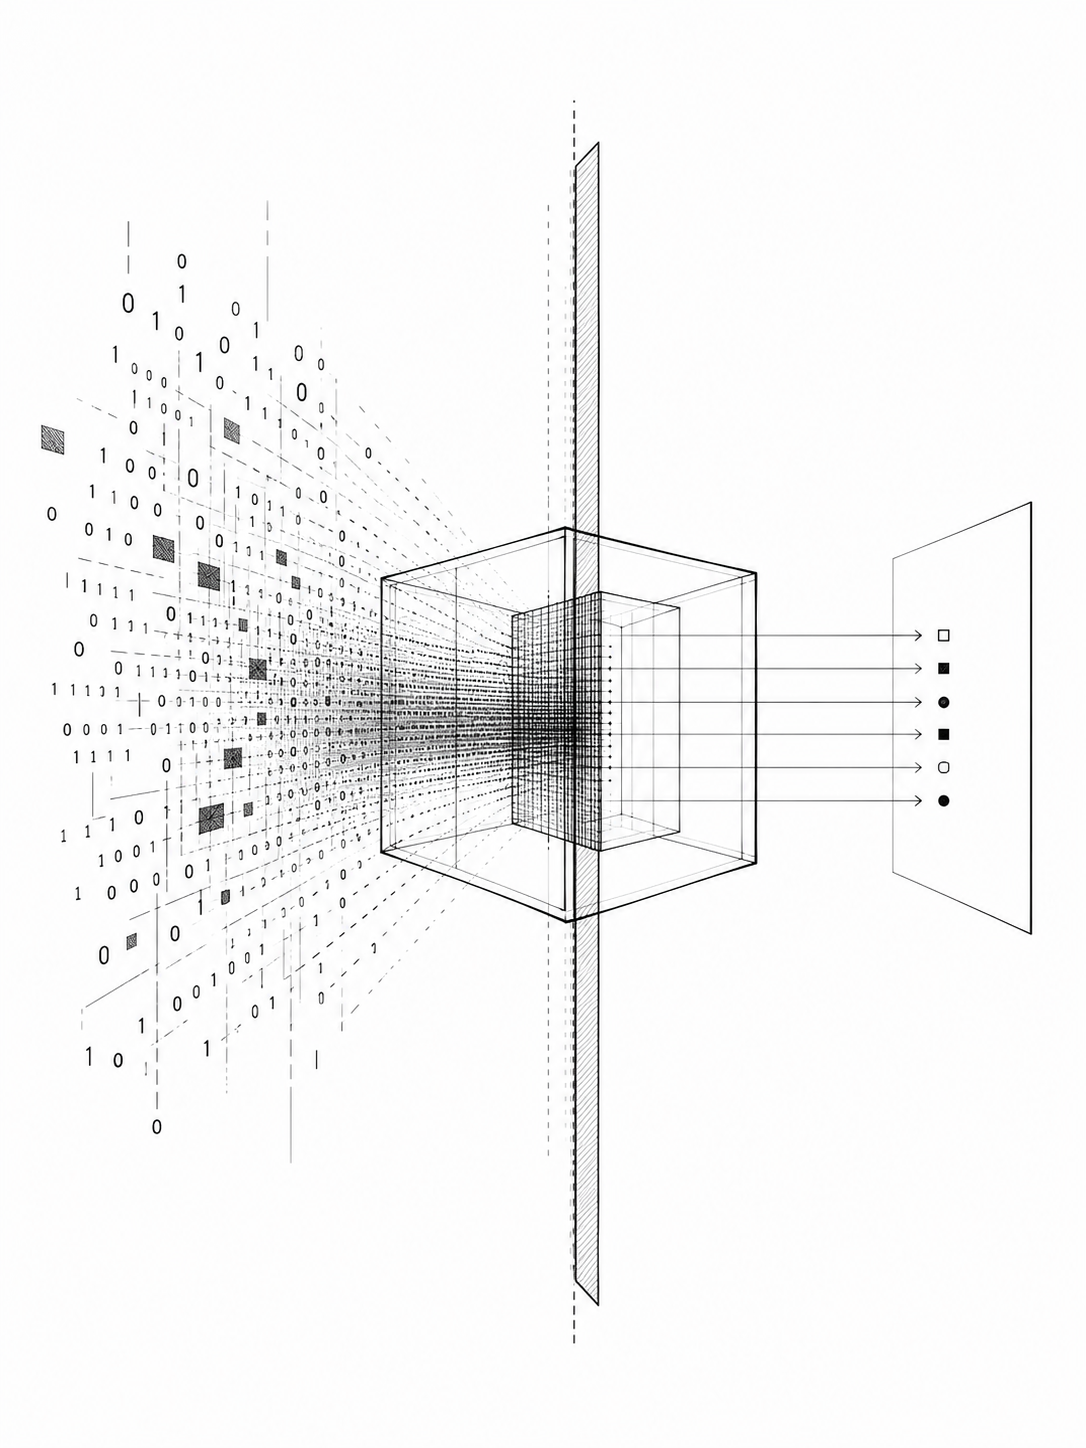
\includegraphics[width=0.6\textwidth]{figures/data_flow_cover_v010.png}}

\begin{document}

\maketitle
\thispagestyle{empty}
\newpage

\pagenumbering{roman} 
\begin{abstract}
The initial parameters for \texttt{audit-probes} are established as a minimal Python artifact for reproducible interrogation across software supply-chain review, telemetry handling, and cloud/API observability. It addresses the practical tension between mission-critical and agent-assisted systems: the need to
produce verifiable audit evidence without expanding the telemetry surface into an operational or adversarial liability. This work reconciles the trade-offs inherent to this dichotomy as an information-resistance problem and proposes ``minimum viable disclosure'' as an architectural principle for bounded, inspectable traces. The current implementation is not a production security platform. It is a deterministic baseline whose evidence consists of module outputs, JSON schemas, and test-log metrics. In the current repository state, eleven of eleven executed tests pass, the executed pass/fail entropy is (0.000000) bits, and the inclusive pass/skip log-outcome entropy is (0.000000) bits. \end{abstract}
\newpage

\pagenumbering{arabic}
\setcounter{page}{1}

\section{Introduction}
Modern technical systems often fail at the boundaries of source-code provenance and deployment, telemetry data versus preprocessing assumptions, in addition to the divide between cloud-provider claims and empirical measurements. The \texttt{audit-probes} artifact investigates whether foundational deterministic probes can make these perimeters more observable without introducing opaque model complexity.

The research question is:

\begin{quote}
Can minimal, active cross-domain audit probes provide reproducible evidence of early-stage systemic fragility before complex failures emerge?
\end{quote}

Observability is established as an active measurement process rather than a passive dashboard property. The aim is not to prove that the probes detects 
all systemic divergence; therefore, the central claim is that a disciplined baseline artifact can convert local observations into structured traces 
that are easier to inspect, validate, and extend.

\section{Theoretical Frame}

\subsection{Adversarial Observability}

In ordinary operations, observability is often framed as the accumulation of logs, telemetry, and internal state. This becomes a double-edged strategy in adversarial settings. A fully transparent system can assist auditors, and simultaneously provide a blueprint for threat actors. Deploying oppositional 
observability as a working frame means that audit attestations should be sufficient for verification, but not expansive in ways that disclose unnecessary internal logic.

\subsection{Information Resistance}

The division between a system's internal state and the externally verifiable evidence available to an auditor constitutes information resistance. Within future autonomous environments, this may be formalized as agentic impedance. While still providing a reproducible control environment for validation stability, the inaugural iteration does not yet claim to measure internal agent cognition. Instead, this report uses Shannon entropy \cite{shannon} for the observed test-log outcome distribution, as defined in Eq. 1:

\begin{equation} 
H(X) = -\sum_{i=1}^{n} p(x_i)\log_2 p(x_i).
\label{eq:shannon_entropy}
\end{equation}

\subsection{Minimum Viable Disclosure}

The proposed design principle is minimum viable disclosure: emit the smallest structured trace that is sufficient to verify the audit event. The prototype prioritizes deterministic JSON outputs, bounded rule logic, schema-defined fields, and reproducible tests. For the subsequent phase, this principle extends to motivate cryptographic anchors and numeric evidence gates rather than unrestricted raw traverse.

\section{Artifact Scope}

The current system contains three modules: \texttt{cyber\_audit}, \texttt{telemetry\_pipeline}, and \texttt{cloud\_probe}.

The cyber module performs rule-based repository checks for possible secret exposure, dependency drift, and unsafe environment-variable access. The telemetry module loads local JSON or CSV telemetry-style records, interpolates missing altitude values, and flags abrupt signal jumps. The cloud module performs repeated endpoint probes and records latency, response size, status codes, and payload fingerprints.

\section{Cross-Domain Architecture}

The cybernetic principles established by Wiener, yield a closed loop of signaling where audit probes serve as the primary feedback for system regulation \cite{wiener}. As shown in Figure \ref{fig:system_architecture}, the interface ensures bounded evidence. 

\begin{figure}[ht]
    \centering
    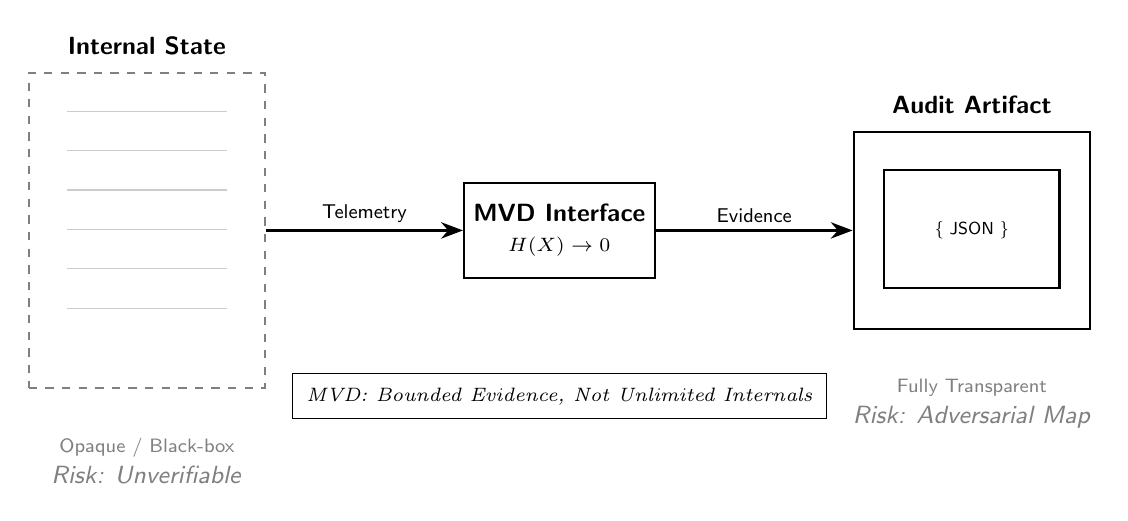
\begin{tikzpicture}[
        node distance=1.5cm and 2.5cm,
        font=\sffamily\small,
        system_box/.style={draw, rectangle, minimum width=3cm, minimum height=4cm, dashed, gray, thick},
        mvd_node/.style={draw, rectangle, fill=white, thick, minimum width=2.2cm, minimum height=1.2cm, align=center},
        trace_box/.style={draw, rectangle, minimum width=3cm, minimum height=2.5cm, thick},
        arrow/.style={-{Stealth[scale=1.2]}, thick}
    ]
        \node[system_box] (system) {};
        \node[above=0.1cm of system] {\textbf{Internal State}};
        
        \foreach \i in {1,...,6}
            \draw[gray!40] ([xshift=0.5cm, yshift=-\i*0.5cm]system.north west) -- ([xshift=-0.5cm, yshift=-\i*0.5cm]system.north east);
    
        \node[mvd_node, right=of system] (mvd) {\textbf{MVD Interface} \\ \scriptsize $H(X) \to 0$};
        
        \node[trace_box, right=of mvd] (trace) {};
        \node[above=0.1cm of trace] {\textbf{Audit Artifact}};
        
        \draw[thick] ([xshift=0.4cm, yshift=-0.5cm]trace.north west) rectangle ([xshift=-0.4cm, yshift=-2cm]trace.north east);
        \node[scale=0.7] at (trace.center) {\{ JSON \}};
    
        \draw[arrow] (system.east) -- (mvd.west) node[midway, above, scale=0.8] {Telemetry};
        \draw[arrow] (mvd.east) -- (trace.west) node[midway, above, scale=0.8] {Evidence};
    
        \node[below=0.5cm of system, align=center, gray] (low) {\scriptsize Opaque / Black-box \\ \textit{Risk: Unverifiable}};
        \node[below=0.5cm of trace, align=center, gray] (high) {\scriptsize Fully Transparent \\ \textit{Risk: Adversarial Map}};
        
        \node[below=1.2cm of mvd, draw, inner sep=5pt, font=\scriptsize\itshape] {
            MVD: Bounded Evidence, Not Unlimited Internals
        };
    \end{tikzpicture}
    \caption{\textbf{Minimum Viable Disclosure Interface.} The pipeline shows the transition from internal state to audit artifacts.}
    \label{fig:system_architecture}
\end{figure}

\section{Methodology}

The artifact follows three methodological constraints. First, every probe must produce inspectable output. Second, assumptions must be surfaced rather than
hidden in preprocessing. Third, validation must be runnable in a constrained local environment for reproducibility that does not depend on privileged infrastructure.

The implementation is intentionally deterministic. Pattern-based checks are used instead of obfuscated anomaly models. Telemetry cleaning records interpolation
assumptions. Cloud probing records simple empirical signals: status, latency, payload size, and response fingerprint. This provides a foundation that can later
be compared with higher-dimensional proposed expansion instrumentation.

\section{Baseline Results}

Environment resolution yields a validation log of eleven discovered tests and eleven executed passes. The distribution has converged to a zero-entropy state. 
For the primary pass/fail behavior, the outcome is calculated using the entropy definition in Equation \eqref{eq:shannon_entropy}:

\begin{equation} 
p(\mathrm{pass}) = 1.0,\quad p(\mathrm{fail}) = 0.0,\quad H_{\mathrm{pass/fail}} = 
-1.0\log_2(1.0) = 0.000000\ \mathrm{bits}.
\label{eq:baseline_results} 
\end{equation}

Because the optional dependency for telemetry is now satisfied within the active interpreter, the inclusive log-outcome distribution is similarly deterministic:

\begin{equation} 
H_{\mathrm{outcome}} = -1.0\log_2(1.0) = 0.000000\ \mathrm{bits}.
\label{eq:distribution} 
\end{equation}

\begin{figure}[htbp]
    \centering
    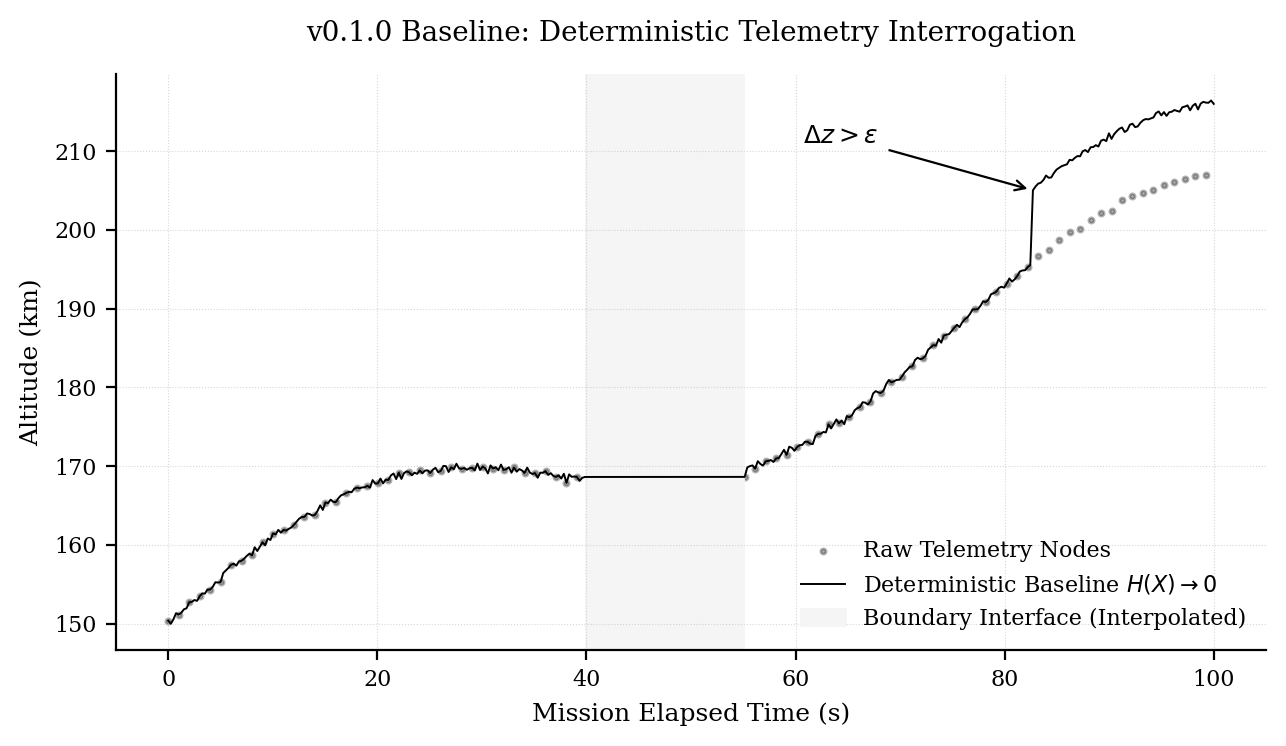
\includegraphics[width=0.95\linewidth]{figures/telemetry_baseline_v010.png}
    \caption{\textbf{Version 0.1.0 Baseline.} Deterministic telemetry interrogation simulated by the \texttt{audit-probes} initial iteration telemetry module. The plot mirrors the technical standards of space systems, demonstrating the interpolation of sparse nodes and the interrogation of systemic divergence ($\Delta z > \epsilon$). Visual artifacts and diagrams were produced through a collaborative synthesis of author-led conceptual sketches and generative tools.}
    \label{fig:telemetry_plot}
\end{figure}

\noindent \textbf{Analysis of the Baseline Plot}

\begin{itemize}
    \item \textbf{Interpolated Boundary:} The shaded region represents the implemented module's capability to maintain a stable structural shape 
even when telemetry nodes are missing. This fulfills the requirement for reproducible interrogation across sparse datasets.
    
    \item \textbf{Signal Jump ($\Delta z > \epsilon$):} The annotation highlights an execution anomaly where a sudden vertical displacement exceeds the minimalist rule-based threshold. This serves as a primary trigger for the \texttt{audit-probes} reporting logic.
    
    \item \textbf{Deterministic Integrity:} The convergence of raw noise into a continuous baseline confirms that the probes act as a feedback mechanism for system regulation, effectively transforming erratic internal states into a citable, zero-entropy pilot study.
\end{itemize}

\begin{table}[htbp] 
   \centering
   \small
   \caption{Implementation matrix and validation results.}
   \label{tab:implementation}
   \begin{tabular*}{\textwidth}{@{\extracolsep{\fill}}
       >{\RaggedRight}p{0.22\linewidth}
       >{\RaggedRight}p{0.14\linewidth}
       >{\RaggedRight}p{0.28\linewidth}
       >{\RaggedRight}p{0.28\linewidth}@{}}
       \toprule
       Core Objective & Feature & v0.1.0 implementation & Future intent \\ \midrule
       Minimal probing for systemic risk & Detection & Pattern matching and deterministic rule logic & ML-assisted anomaly detection and access-gated repository probes \\ \addlinespace
       Probabilistic telemetry pipeline & Telemetry & Local JSON artifacts and deterministic cleaning assumptions & Higher-dimensional telemetry streams and KTH-adjacent fixtures after access approval \\ \addlinespace
       Control-theoretic system view & Risk analysis & Static severity and impact classes & Probabilistic risk modeling using \(R=P\times I\) \\ \bottomrule
   \end{tabular*}
\end{table}

The following analysis evaluates the current implementation (detailed as version 0.1.0 in Table \ref{tab:implementation}) against its planned enhancements (version 0.2.0). Table 2 summarizes the existing system's audit results. The zero-entropy pass/fail state confirms the deterministic reliability of the core logic, utilizing logarithmic measures to quantify informational uncertainty.

\begin{table}[htbp]
    \centering
    \caption{Version 0.1.0 baseline performance summary (Resolved Environment).}
    \label{tab:performance}
    \small
    \begin{tabularx}{\textwidth}{l X r}
        \toprule
        \textbf{Metric category} & \textbf{KPI} & \textbf{Baseline value} \\ \midrule
        Operational integrity & Test execution success rate & 100.000000\% \\
        Operational integrity & Optional-dependency skip rate & 0.000000\% \\
        Validation stability & Pass/fail entropy & 0.000000 bits \\
        Validation stability & Inclusive log-outcome entropy & 0.000000 bits \\
        Security and compliance & Log integrity state & JSON emitted \\
        Security and compliance & Bundled-target findings & 0 findings \\ \bottomrule
    \end{tabularx}
\end{table}

\section{Schemas and Reproducibility} \label{sec:reproducibility}

The repository provides JSON schemas for the cyber audit report, cloud probe summary, and telemetry sample records. These schemas define a foundational evidence 
contract: formalizing required fields, numeric bounds, enumerated severity levels, and fingerprint formats. The validation suite utilizes dependency-free sanity tests to ensure that the contract and Python module outputs remain aligned. This schema layer establishes the current trace discipline; while it does not yet implement signed attestations, it secures a stable structural shape for 
future cryptographic anchoring. 

\section{Discussion}

\subsection{The Glasshouse Dilemma}

The central policy and engineering tension is the glasshouse dilemma. A system that exposes all internal state, offers ease of inspection but invites unauthorized mapping and exploitation. Conversely, a black-box system shields internal logic while leaving auditors unable to verify behavior. Minimum viable disclosure resolves this conflict by providing bounded evidence without exposing unlimited internals.

\begin{figure}[htbp]
    \centering
    \vspace{1em}
    
    \begin{minipage}{0.8\linewidth}
        \centering
        \small
        \begin{equation}
            H(X) = -\sum_{i=1}^{n} p(x_i)\log_2 p(x_i)
        \end{equation}
        \begin{equation}
            H_{\mathrm{v0.1.0}} = 0.000000 \, \mathrm{bits} \label{eq:baseline_val}
        \end{equation}
    \end{minipage}
    
    \vspace{1em}
    
    \caption{\textbf{The Glasshouse Dilemma.} Information resistance is represented as the divide between internal system state and deterministic audit artifacts. The prototype establishes a zero-entropy baseline as formalized in Equation \ref{eq:baseline_val}.}
    \label{fig:glasshouse_dilemma}
\end{figure}

\subsection{Mapping to Security Controls}

The current system aligns most naturally with audit and integrity goals: deterministic records, reproducible execution, bounded findings, and stable schemas. It addresses the tension separating mission-critical and agent-assisted systems as a fundamental security engineering problem where designers must protect the right data in the right way \cite{anderson}. It should not be described as satisfying a complete National Institute of Standards and Technology (NIST) System and Information Integrity control family, that focuses on vulnerability remediation, in addition to protection against the intentional, inadvertent, and incidental threats to a system's dependability. A safer interpretation is that it provides a minimal technical substrate for future auditability and integrity work.

\section{Access-Gated version 0.2.0 Targets}

Within the scope of the preliminary release, public contributions to KTH Royal Institute of Technology and the CHAINS research project about "Consistent Hardening and Analysis of Software Supply Chains"\footnote{Project page: \url{https://github.com/chains-project}.} could not be verified as evidence for the baseline. Specific external repositories are therefore not referred to as results in Section~\ref{sec:reproducibility}. Adjacent projects stemming from KTH Rymdcenter and other Space Agencies are treated as access-gated candidates. Integration in the future enhanced system is contingent upon formal recording of the repository URL, access permissions, commit hashes, licensing, and defined audit scope.

\section{Limitations}

The artifact is built upon an intentionally deterministic and rule-based architecture. Current detection logic prioritizes string and regular-expression patterns over semantic program analysis to ensure a transparent, high-integrity baseline. Telemetry cleaning remains in an exploratory phase and is not yet positioned for high-stakes production reconstruction; similarly, cloud latency measurements are presented as raw data prior to network normalization. \texttt{audit-probes} is therefore established strictly as a reproducibility and traceability foundation, rather than an exhaustive performance benchmark.

The theoretical scope is similarly disciplined and bounded. Agentic impedance, entropy-gated execution, and cryptographic state anchors are designated 
as optimized variant research directions. These trajectories will remain theoretical until the repository incorporates the direct supporting logs, 
implementations, and validation tests required to promote them into current system.

\section{Roadmap}

The future state focuses on graduating the initial \texttt{audit-probes} into an active security protocol:

\begin{enumerate}
\item Transition from ordinary schemas to cryptographically anchored 
attestations to ensure non-repudiation.
\item Integrate probabilistic risk modeling ($R=P \times I$) to complement 
the existing deterministic baseline tests.
\item Quantify entropy and stability metrics against live systemic divergence 
within actual execution traces.
\end{enumerate}

\section{Conclusion}

Audit probes demonstrate a compact approach to cross-domain technical interrogation. Explicit assumptions, deterministic outputs, schema-defined evidence, and a reproducible baseline validation implement a foundational value. The larger theory is a direction of odyssey: auditable infrastructure should produce enough evidence to verify behavior without yielding its internal logic as adversarial coordinates.

\begin{thebibliography}{9}

\bibitem{anderson}
Ross Anderson.
\newblock \textit{Security Engineering: A Guide to Building Dependable Distributed Systems}.
\newblock Wiley, 3rd edition, 2020. 

\bibitem{shannon}
Claude E. Shannon.
\newblock A mathematical theory of communication.
\newblock \textit{Bell System Technical Journal}, 27(3):379--423 and 27(4):623--656, 1948.

\bibitem{wiener}
Norbert Wiener.
\newblock \textit{Cybernetics: Or Control and Communication in the Animal and the Machine}.
\newblock MIT Press, 1948. 

\end{thebibliography}

\end{document}
